\chapter{Hardware} \label{chap:methods}
Na obrázku \cref{fig:hardware_diagram} je zobrazen použitý hardware v závislosti na měřených veličinách. V projektu chytré domácnosti jsem využil celkem 5 samostatných microchipů ESP8266, 7 čidel pro měření fyzikálních veličin a jeden počítač Raspbery Pi, který slouží primárně jako databázový server a webserver.

\begin{figure}[H]
  \centering
  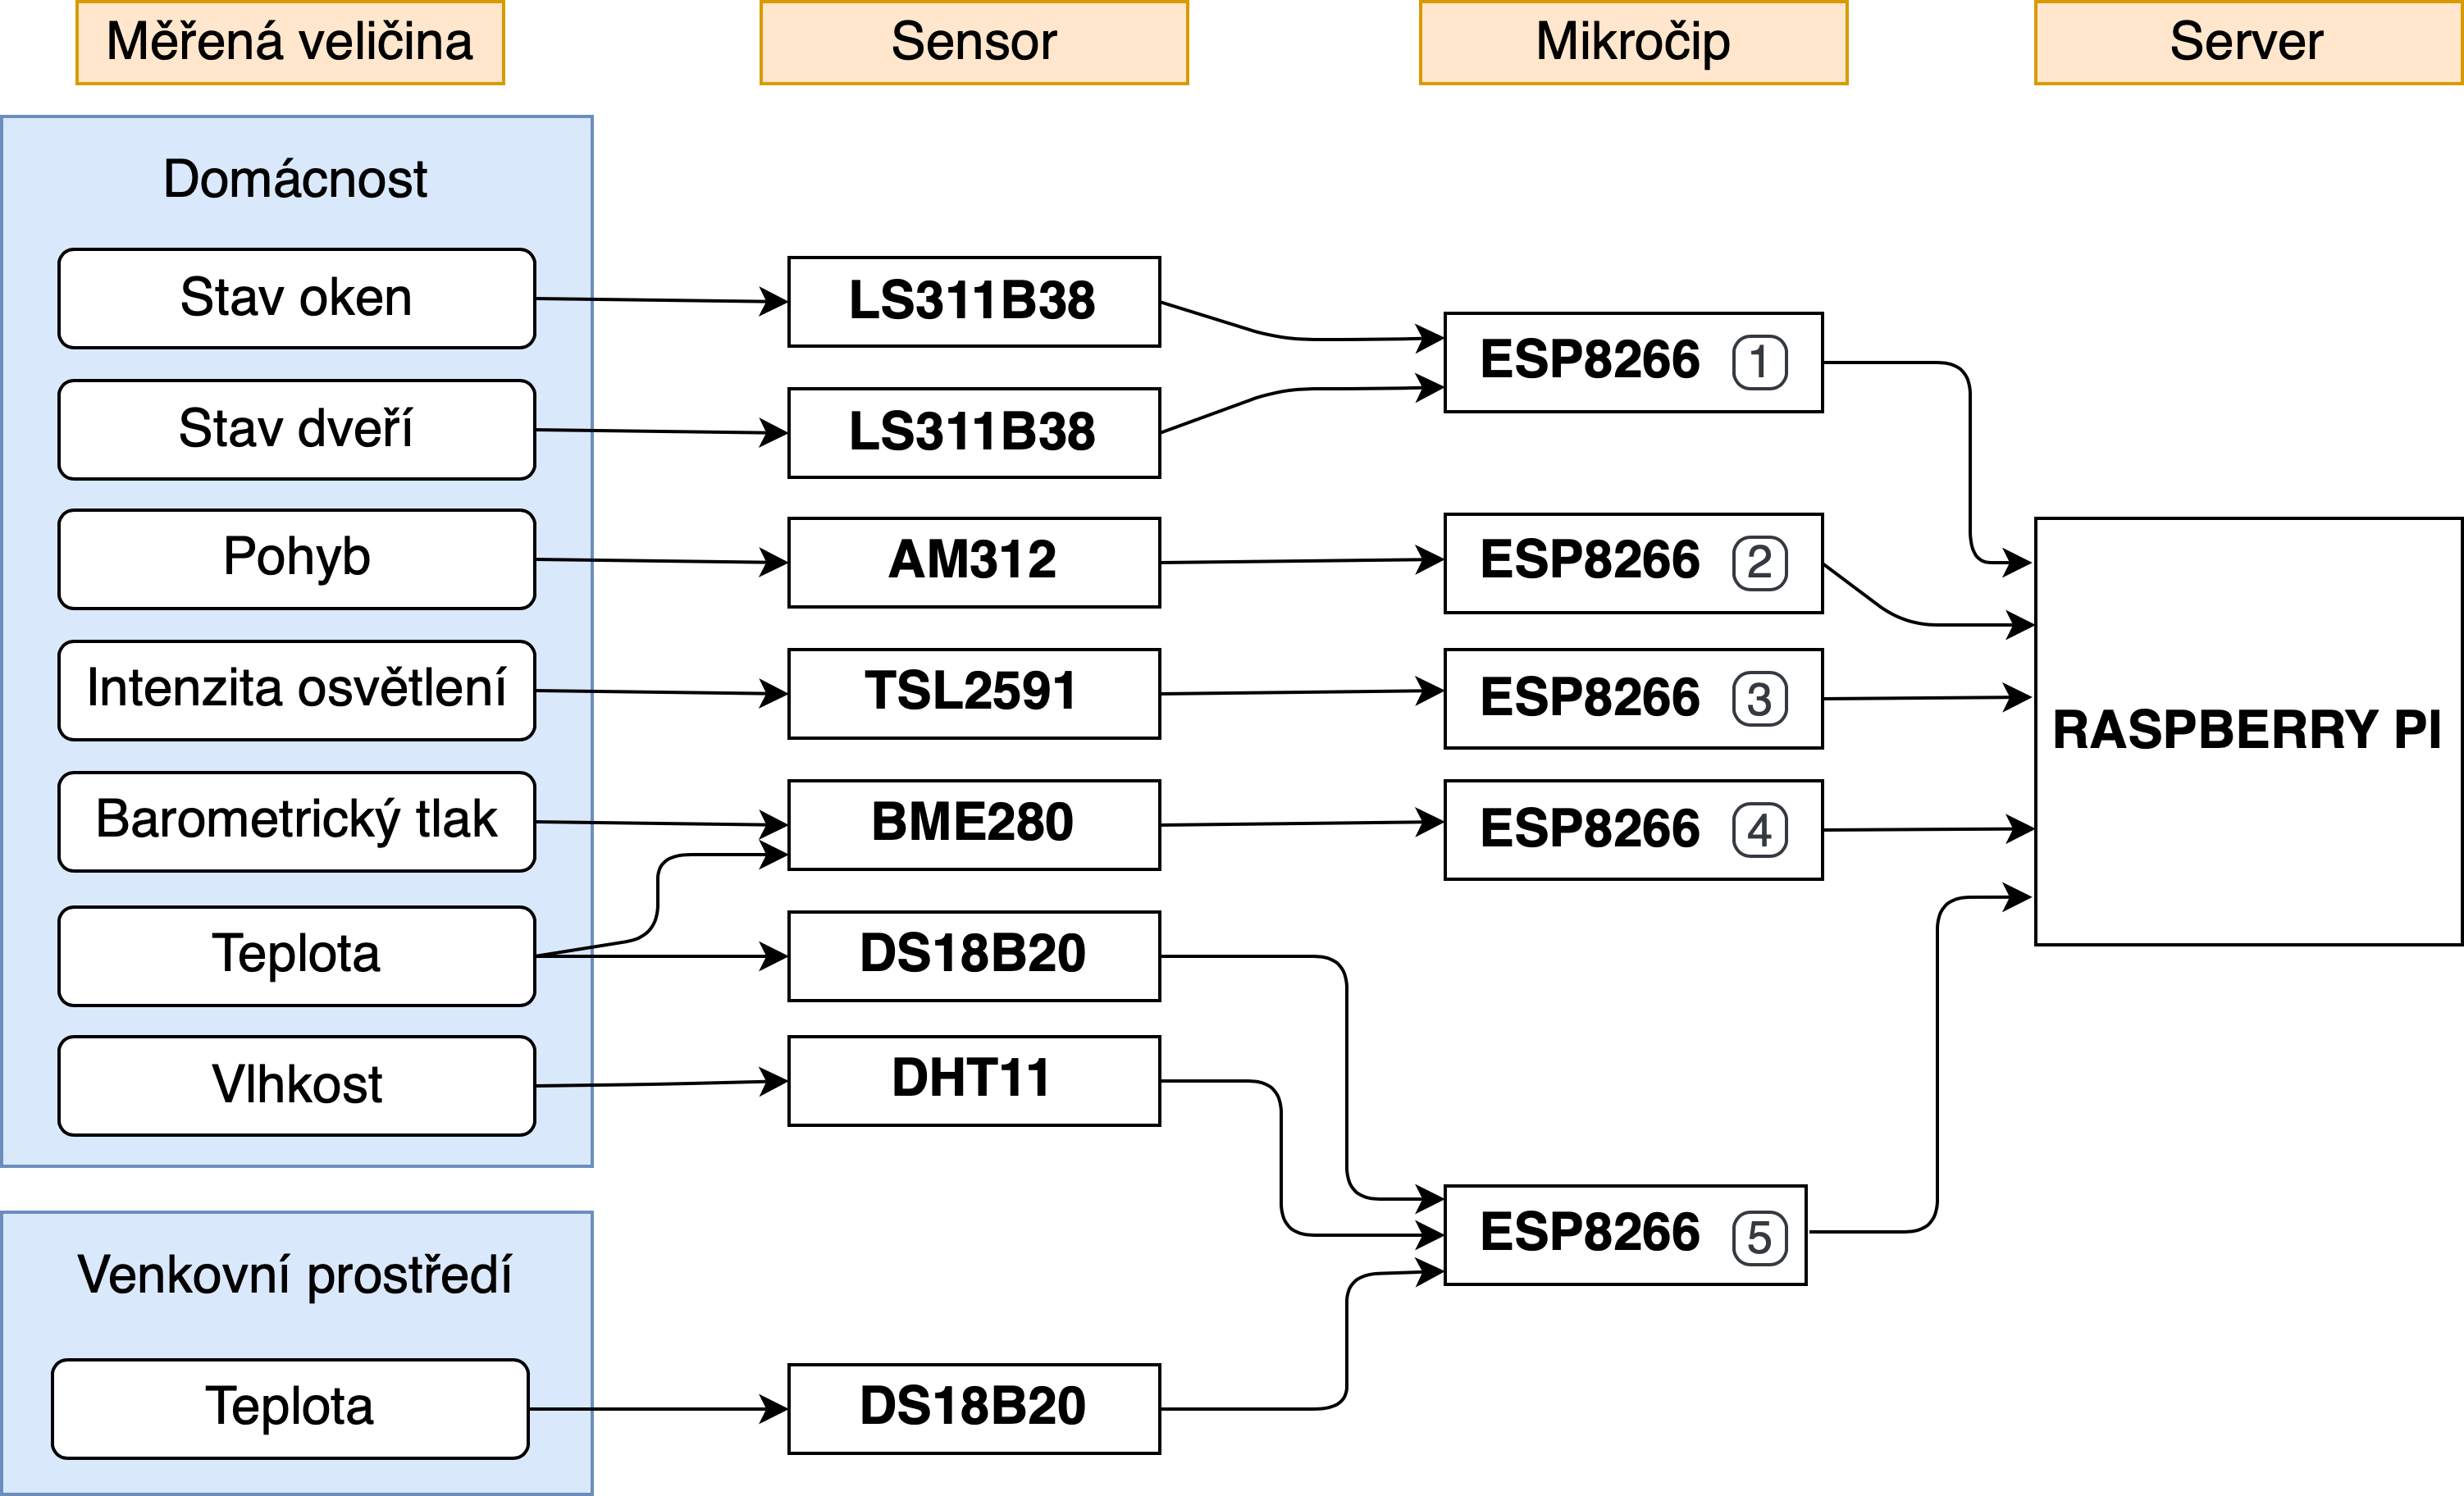
\includegraphics[width=1 \textwidth]{hardware_diagram.png}
  \caption{Vztahy mezi použitým hardwarem a měřenými veličinami}
  \label{fig:hardware_diagram}
\end{figure}



\section{ESP8266} \label{sec:example_xor}

Fyzická realizace čidel \\
ESP programováno v MicroPythonu (proč, výhody, nevýhody oproti Arduinu) \\
Seznámení s microchipem ESP8266 (proč zrovna toto ESP, flashování firmwaru, přístup k souborům na microchipu přes mpfshell, pricip programování microchipu) \\
Popis funkčnosti a možností ESP (GPIO piny, analogové, digitální vstupy/ výstupy, WiFi konektivita, ...) \\
Zapojení (obvodu na breadboardu) a komunikace s čidly vhodnými pro využití v projektu chytré domácnosti \\
Otestování funkcionality a spolehlivosti senzorů pro využití v chytré domácnosti  \\
Vytvoření designu a vytvoření pevného obvodu - ESP + čidlo na PCB desce \\
Popis logiky komunikace mezi ESP, jednotlivými čidly a odesíláním zpráv (prvně připojit k wifi -> načíst hodnotu měřené veličiny -> v případě, že hodnota OK -> odeslat zprávu na broker -> uspat se) \\
Naprogramování logiky ESP - dva použité principy (periodické odesílání zpráv nebo odesílání zpráv založené na události) \\
Objektově orientovaná struktura kódu na ESP - boot.py, main.py, config.py, mqttclient.py, skript pro načítání dat z konkrétního senzoru (důraz kladen na objektové programování - přehlednost kódu, snadné změny, konfigurační soubor pro nastavení vstupních parametrů, univerzální kód pro všechna esp, snadná rozšiřitelnost kódu do budoucna, snadná implementace dalších senzorů, ...) \\

\begin{figure}[H]
  \centering
  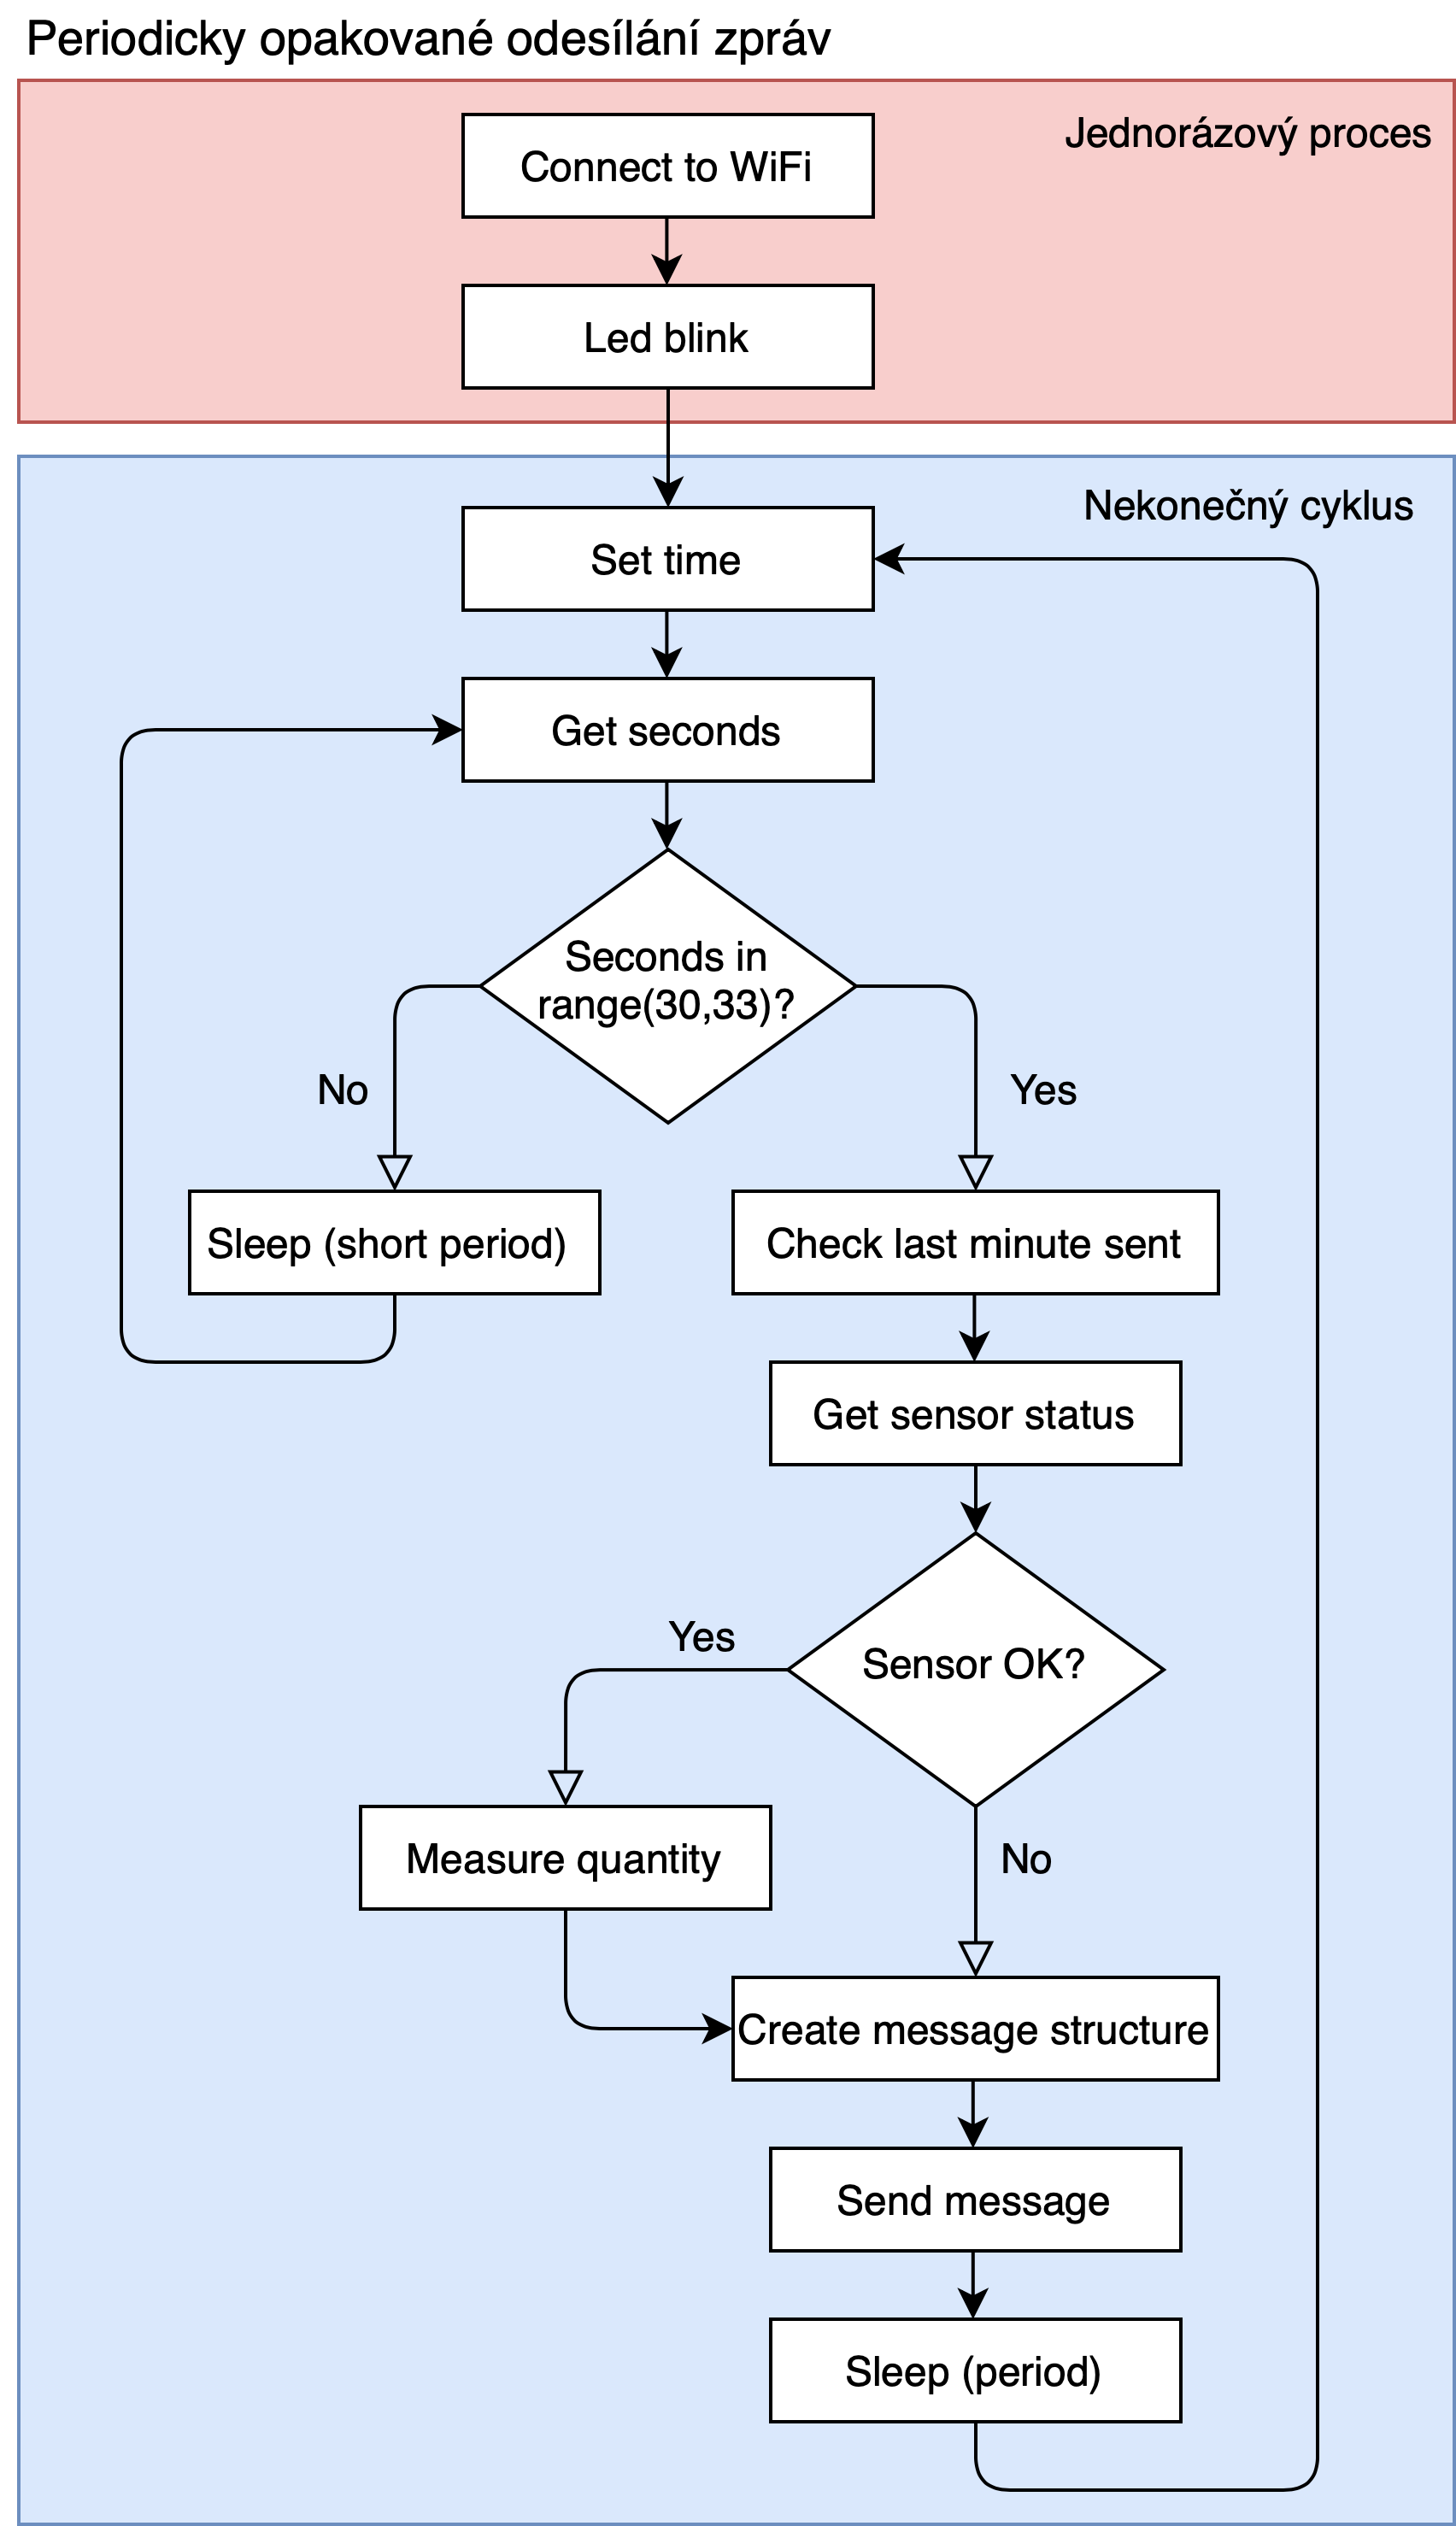
\includegraphics[width=1 \textwidth]{esp_periodical_diagram.png}
  \caption{Diagram periodicky opakovaného odesílání zpráv}
  \label{fig:methods:transfer_functions}
\end{figure}

\begin{figure}[H]
  \centering
  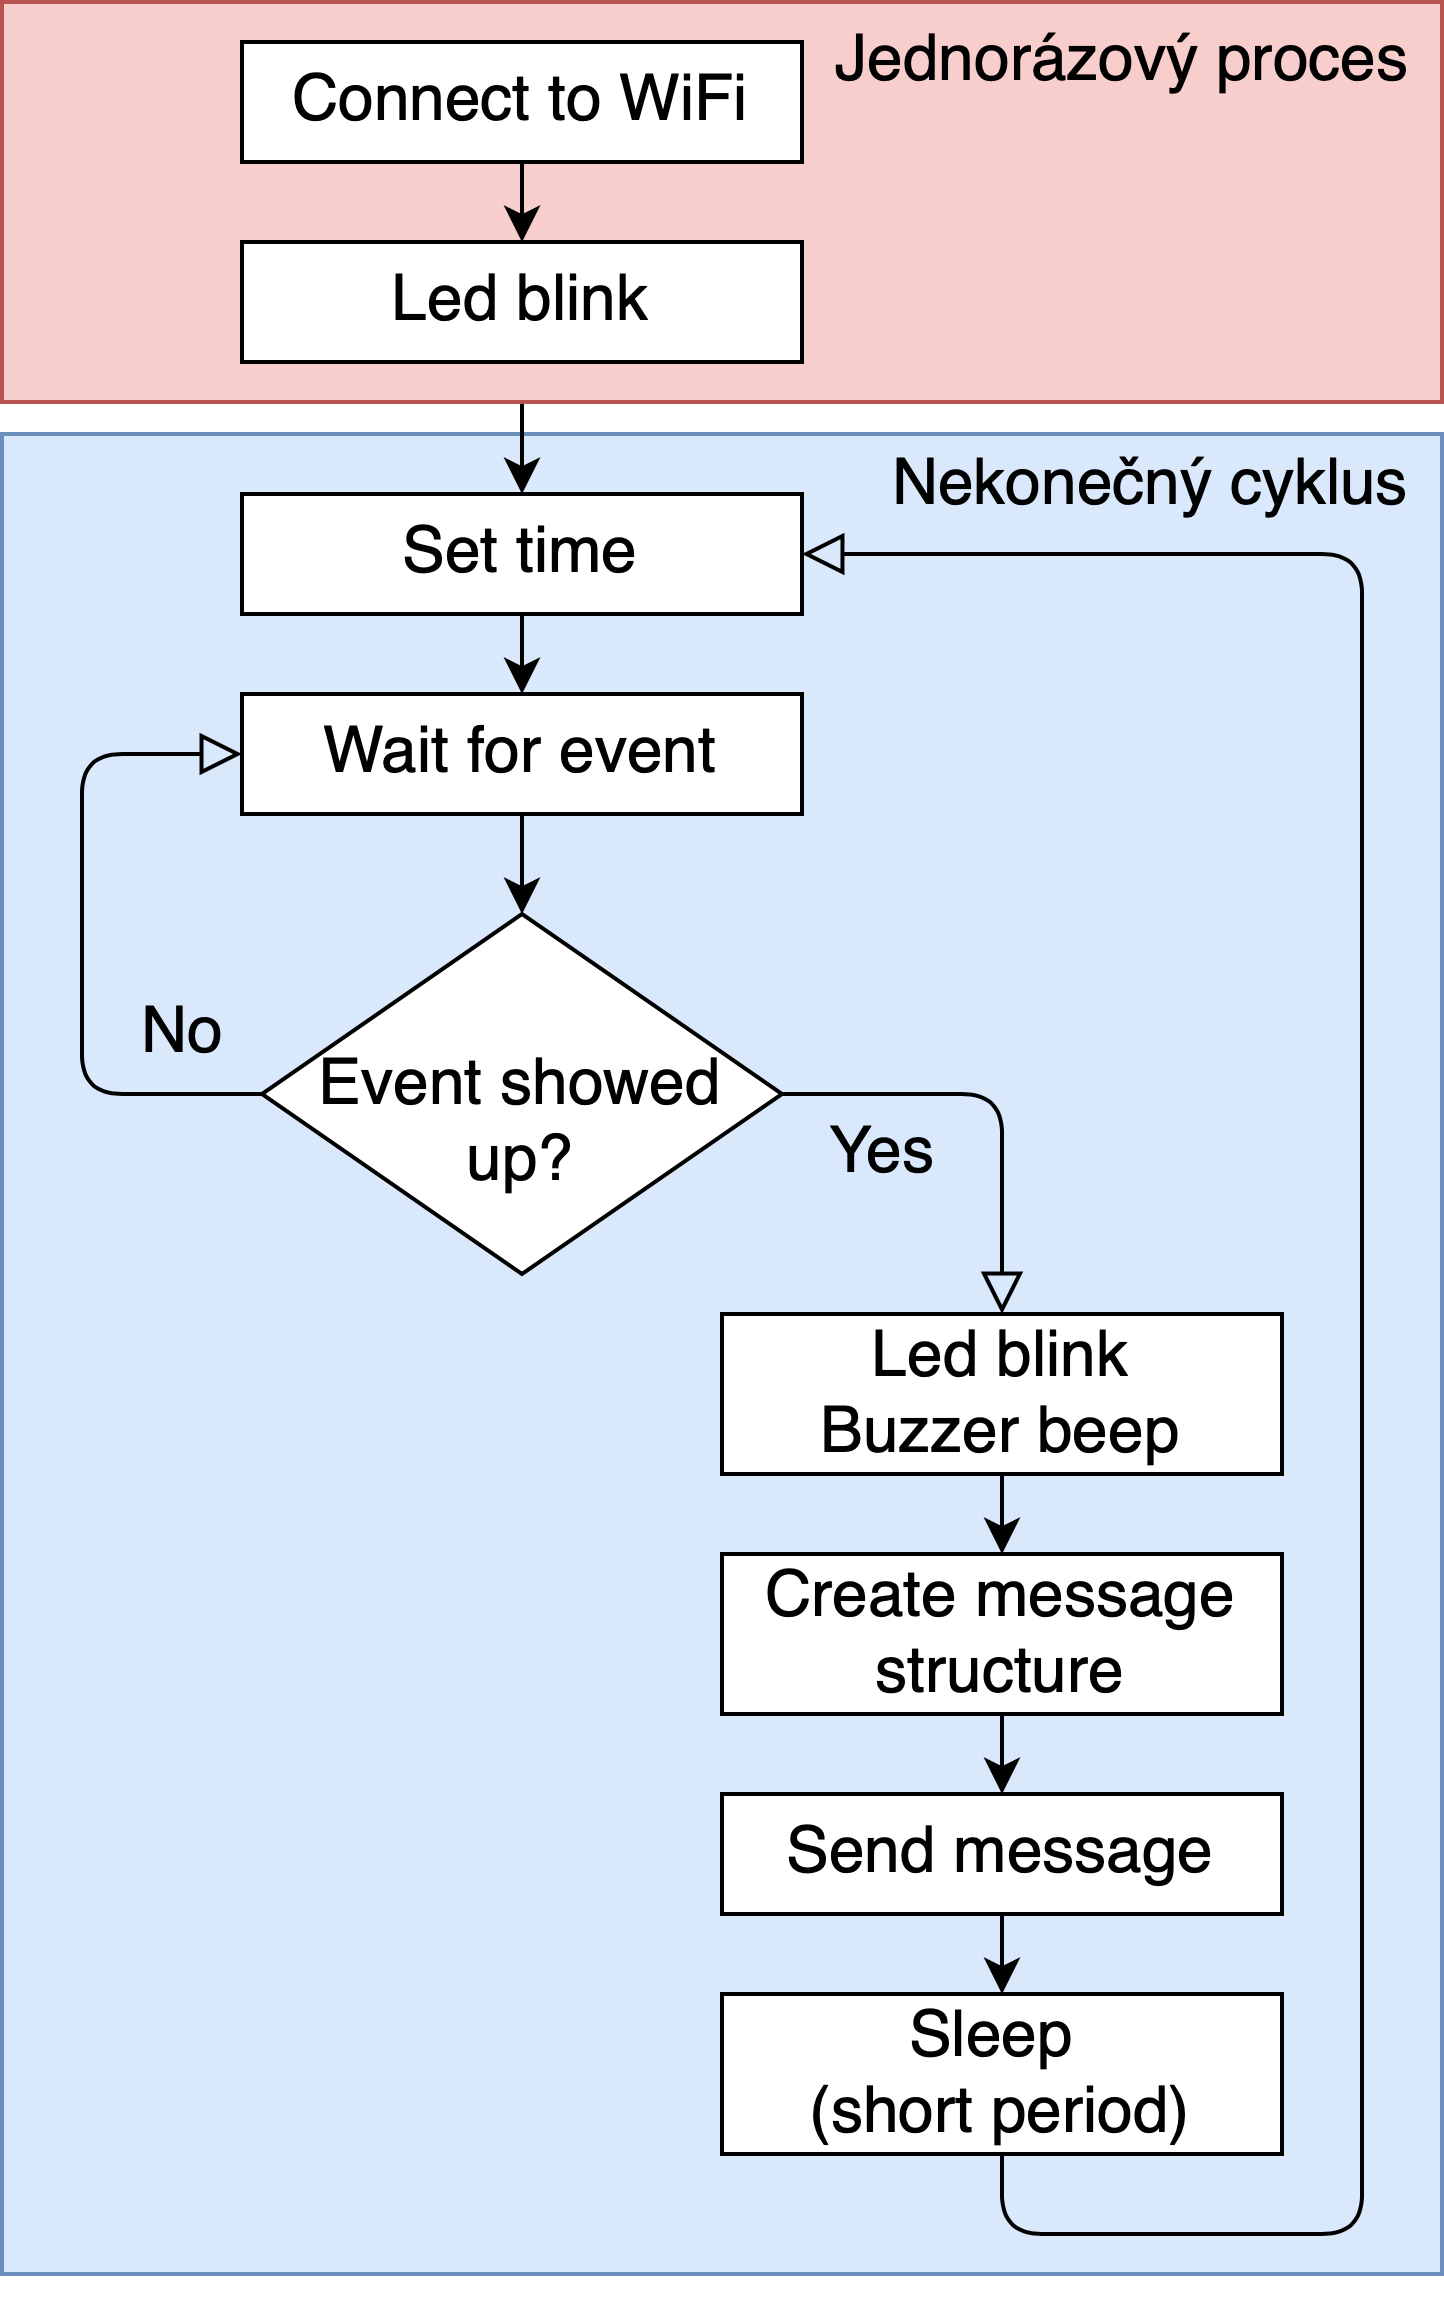
\includegraphics[width=1 \textwidth]{esp_event_based_diagram.png}
  \caption{Diagram odesílání zpráv na základě vzniku události}
  \label{fig:methods:transfer_functions}
\end{figure}

\begin{figure}[H]
  \centering
  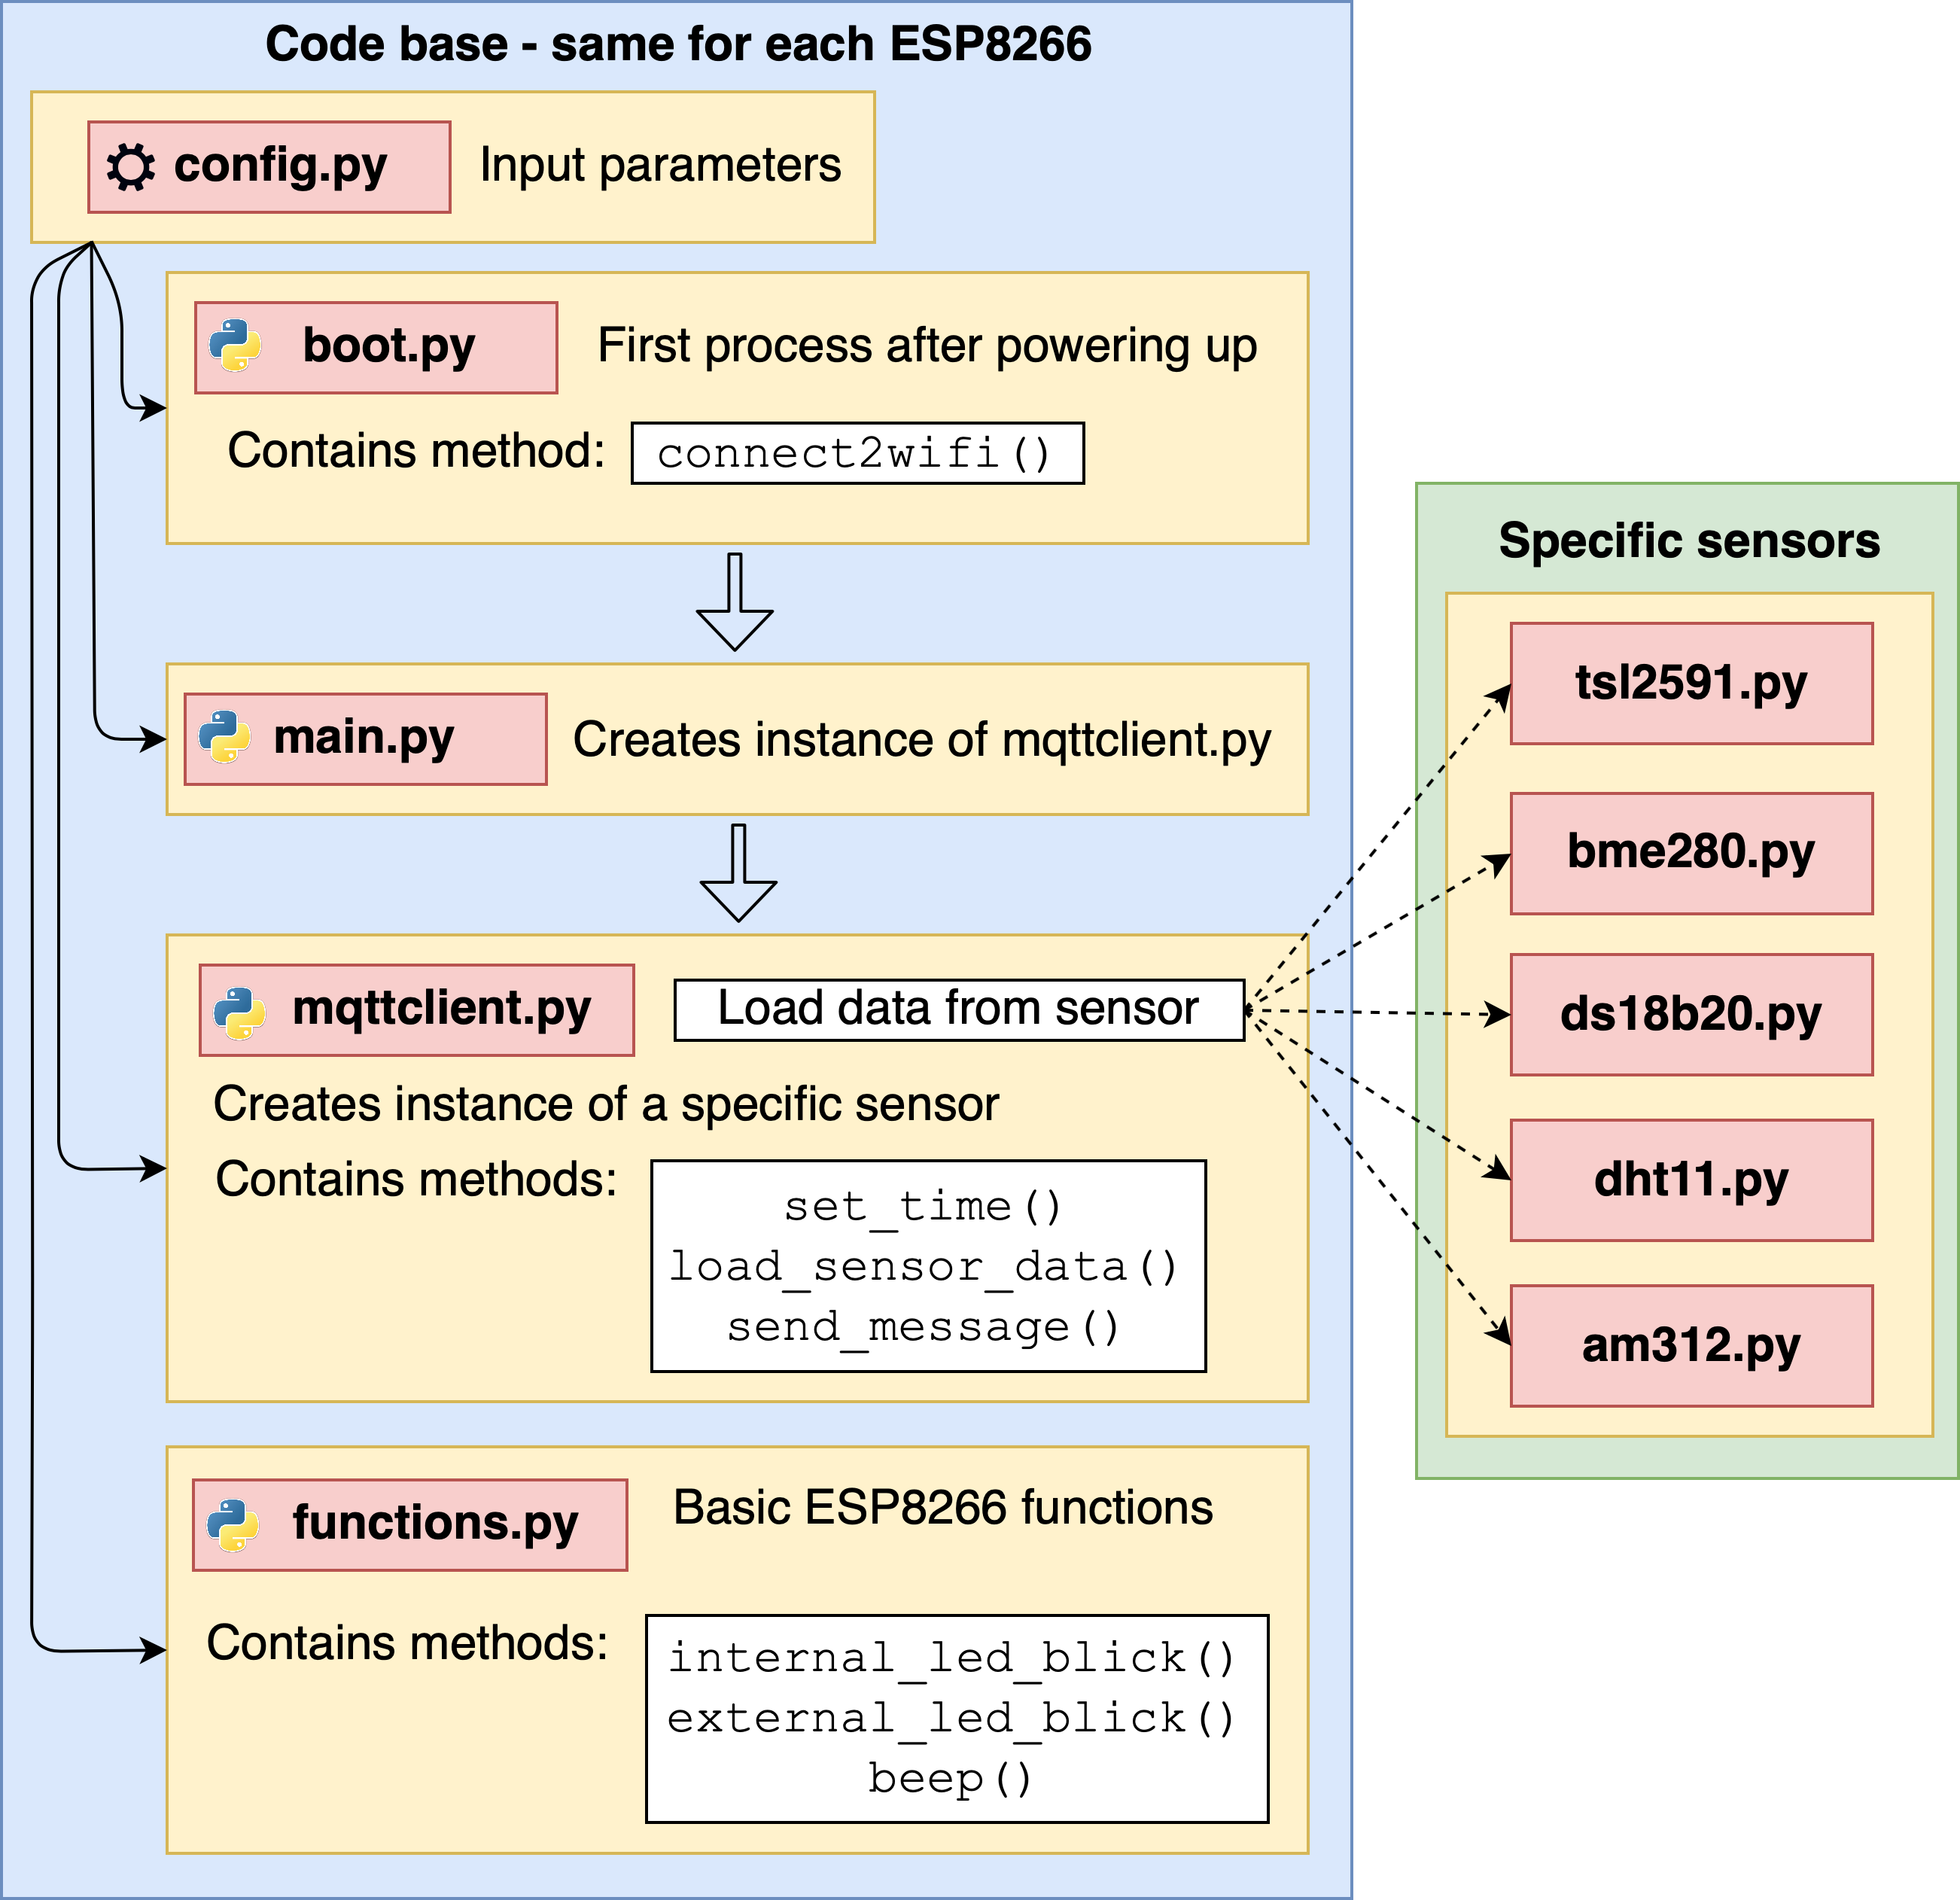
\includegraphics[width=1 \textwidth]{esp_code_architecture.png}
  \caption{Diagram architektury kódu na microchipu ESP8266}
  \label{fig:methods:transfer_functions}
\end{figure}

\section{Senzory} \label{sec:example_xor}

V projektu chytré domácnosti bylo použito celkem 7 senzorů pro měření fyzikálních veličin ... \\
Které veličiny měřeny (využití naměřených hodnot, smysl měřených veličin, ...) \\
Proč vybrány tyto konkrétní senzory \\

\subsection{DS18B20}

esp-temphumid \\
Senzor pro měření teploty \\
Základní informace o senzoru - rozsah měření, přesnost, napájení, způsob komunikace, životnost, spolehlivost, ... \\
Více variant - vnitřní, venkovní \\
Obvod zapojení - esp, senzor, rezistor, napájení obvodu na PCB desku, umístění v místnosti \\
Zprovoznění komunikace s teplotními čidlem ds18b20 (room a outside) \\
Schéma zapojení senzoru, esp8266 a dalších periferií (led světlo, bzučák, ...) \\
Fotka reálného zkonstruovaného čidla \\

Senzor DS18B20 je jedním z nejdostupnějších senzorů použitých v projektu chytré domácnosti ...

\subsection{DHT11}

esp-temphumid \\
Senzor pro měření teploty a  vlhkosti v místnosti \\
Základní informace o senzoru - rozsah měření, přesnost, napájení, způsob komunikace, životnost, spolehlivost, ... \\
Využití měřených veličin (používáme pouze naměřenou vlhkost, protože teplota má oproti ds18b20 nebo bme280 menší přesnost, ...) \\
Obvod zapojení - esp, senzor, rezistor, napájení obvodu na PCB desku, umístění v místnosti \\
Zprovoznění komunikace s vlhkostním čidlem dht11\\
Schéma zapojení senzoru, esp8266 a dalších periferií (led světlo, bzučák, ...) \\
Fotka reálného zkonstruovaného čidla \\

Senzor DHT11 je ...

\subsection{TSL2591}

esp-lux \\
Čidlo pro měření intenzity osvětlení \\
Základní informace o senzoru - rozsah měření, přesnost, napájení, způsob komunikace, životnost, spolehlivost, ... \\
Obvod zapojení - esp, senzor, rezistor, napájení obvodu na PCB desku, umístění v místnosti \\
Zprovoznění komunikace se senzorem tsl2591 \\
Schéma zapojení senzoru, esp8266 a dalších periferií (led světlo, bzučák, ...) \\
Fotka reálného zkonstruovaného čidla \\

Senzor TSL2591 je ...

\subsection{BME280}

esp-pressure \\
Čidlo pro monitorování vnitřní teploty a barometrického tlaku \\
Základní informace o senzoru - rozsah měření, přesnost, napájení, způsob komunikace, životnost, spolehlivost, ... \\
Obvod zapojení - esp, senzor, rezistor, napájení obvodu na PCB desku, umístění v místnosti, alternativní senzory \\
Zprovoznění komunikace s čidlem bme280 \\
Schéma zapojení senzoru, esp8266 a dalších periferií (led světlo, bzučák, ...) \\
Fotka reálného zkonstruovaného čidla \\

Senzor BME280 je ...

\subsection{AM312}

esp-pir \\
Čidlo pro monitorování pohybu v místnosti \\
Základní informace o senzoru - rozsah měření, přesnost, napájení, způsob komunikace, životnost, spolehlivost, ... \\
Obvod zapojení - esp, senzor, rezistor, napájení obvodu na PCB desku, umístění v místnosti, alternativní senzory - potíže s čidlem hc-sr501\\
Zprovoznění komunikace se senzorem am312 \\
Schéma zapojení senzoru, esp8266 a dalších periferií (led světlo, bzučák, ...) \\
Fotka reálného zkonstruovaného čidla \\

Senzor AM312 je ...

\subsection{LS311B38}

esp-magnet \\
Čidlo pro monitorování stavu dveří a oken \\
Základní informace o senzoru - rozsah měření, přesnost, napájení, způsob komunikace, životnost, spolehlivost, ... \\
Obvod zapojení - esp, senzor, rezistor, napájení obvodu na PCB desku, umístění v místnosti \\
Zprovoznění komunikace s magnetickým senzorem ls311b38 \\
Schéma zapojení senzoru, esp8266 a dalších periferií (led světlo, bzučák, ...) \\
Fotka reálného zkonstruovaného čidla \\

Senzor LS311B38 je ...

\section{Raspberry Pi} \label{sec:example_xor}

Co je to Raspberry Pi \\
Výhody, nevýhody oproti klasickému pc (výpočetní výkon, spotřeba proudu, ... ) \\
Využití v projektu chytré domácnosti - MQTT broker, databázový server, webserver, klasifikace příchozích zpráv \\
Výhody, nevýhody univerzálního použití Raspberry Pi pro několik účelů, ... \\

\chapter{Síťová komunikace a databáze} \label{chap:methods}

Smyslem zkonstruovaných čidel je jejich snadná implementace do bytu či domu. \\
ESP8266 potřebuje jen napájení, celá komunikace mezi microchipem a brokerem probíhá po WiFi \\

\section{Protokol MQTT} \label{sec:example_xor}

Co je to protokol MQTT (vznik, využití) \\
Proč zrovna tento protokol \\
Princip použití protokolu MQTT (v síti je broker, který čeká na příchozí zprávy, ostatní zařízení jsou v módu publish - odesílají zprávy na broker, hierarchie zpráv, ...) \\
Zprovoznění komunikace přes MQTT \\ 
Sestavení struktury zpráv + identifikátorů čidel (popis jednotlivých atributů ve zprávě, proč jedno esp může posílat více zpráv do různých topiců, popis zvolené hierarchie topiců, ...) \\
Popis logiky odesílání zpráv z ESP - ESP odešle zprávu periodicky vždy v polovině minuty (např.: 14:30:30, 14:31:30, ... ) - lehké nepřesnosti způsobené dobou načítání dat ze senzorů, ... \\

\section{Ukládání dat do databáze} \label{sec:example_xor}

Základní princip databáze, proč jsme se rozhodli pro použití databáze,  ... \\
Co je MongoDB (určení, využití, funkčnost, ... ) \\
Ukládání hodnot měřených veličin do MongoDB \\

\chapter{Diagnostika a detekce anomálií} \label{chap:methods}

Proč řešit diagnostiku čidel v rámci chytré domácnosti, ... \\
Úvod do detekce anomálií, základní principy, smysl využití, ... \\
Diagnostika a detekce anomálií v projektu chytré domácnosti probíhá na 3 úrovních ... \\

\section{Detekce chyb na úrovni ESP8266} \label{sec:example_xor}

První a nejnižší úroveň diagnostiky jednotlivých senzorů \\
Implementace detekce chyb na úrovni samotného microchipu \\
Popis základního principu - při načítání ze dat ze senzoru čidlo pozná, když je senzor nefunkční - nevrací  žádné hodnoty a ESP pošle info o nefunkčním senzoru) \\
Robustnost - odolnost ESP vůči výpadkům senzorů - esp nespadne kvůli nefunkčnímu senzoru, jen změní status zprávy, ... \\
Nonstop provoz - senzory lze k ESP připojovat a odpojovat v reálném čase bez nutnosti vypínání nebo restartu microchipu, pokud senzor v jakémkoliv časovém okamžiku odpojím - změní se status zprávy na "error", ve chvíli kdy senzor zase připojím na desku - esp začne měřit a posílat, ... \\

\section{Detekce anomálií na základě klasifikace} \label{sec:example_xor}

Implementace funkcí scikit-learn pro natrénovaní modelů \\
Nastavení modelu a natrénování modelů pro jednotlivé veličiny \\
Porovnání schémat natrénovaných modelů \\
Implementace do projektu - klasifikace jednotlivých příchozích zpráv (přidání atributu "classification" do každé zprávy)
Implementace detekce anomálií přijatých zpráv na základě rozhodnutí klasifikace - klasifikace 1 nebo -1 (1 v případě, že přijatá zpráva svou hodnotou "odpovídá" natrénovanému modelu, -1 v případě, že se vychyluje od natrénovaného modelu) \\
Přenos této informace o klasifikaci do webového rozhraní \\

\section{Diagnostika stavu čidel na serveru} \label{sec:example_xor}

Implementace detekce anomálií na úrovni serveru (brokeru) \\
Implementace funkce sensor-check() \\
Periodická kontrola odesílání zpráv jednotlivých čidel - pokud čidlo z neznámého důvodu neodešle zprávu nebo pokud se zpráva nepřenese k brokeru - informace o anomálii se přenese do webového rozhraní \\
Vysvětlení stavů čidel - 3 možné stavy čidla - ok, value-error, error \\

Závěr diagnostiky: kontrola stavu jednotlivých čidel + kontrola věrohodnosti posílaných hodnot + kontrola pravidelnosti odesílaných zpráv


\chapter{Webové rozhraní} \label{chap:methods}

Důvod využití webové vizualizace \\ 
Frontend - popis struktury webu - proč 3 záložky, popis Overview, Analytics, About, ... \\
Smysl Overwiev - nonstop zobrazení dat na monitoru, ... \\
Přijímání aktuálních zpráv z ESP bez nutnosti refresh stránky přes websockets - co je websockets, důvod využití této technologie, alternativa v podobě json souboru - nevýhody, ... \\
Backend - z hlediska programování - jeden soubor engine.py, který zajišťuje serverování webové stránky, ukládání dat do databáze, sensor check, ... \\

Zajištění integrity celého webu (nově přijaté zprávy se propisují na web, po znovunačtení se ihned ukazují poslední přijaté hodnoty - má smysl hlavně u neperidicky posílaných veličin, ...) \\



